\chapter{Kajian Pustaka}

\section{Wisata dan Pariwisata}
Wisata adalah kegiatan perjalanan yang dilakukan oleh seseorang atau sekelompok orang dengan mengunjungi tempat tertentu untuk tujuan rekreasi, pengembangan pribadi, atau mempelajari
keunikan daya tarik wisata yang dikunjungi dalam jangka waktu sementara.

Pariwisata adalah berbagai macam kegiatan wisata dan didukung berbagai fasilitas serta layanan yang disediakan oleh masyarakat, pengusaha, pemerintah dan Pemerintah Daerah\cite{uupariwisata}.

\section{Recommender System}

\textit{Recommender system} (RS) adalah kakas dan teknik yang digunakan untuk mendapatkan sebuah saran atau rekomendasi item yang dapat digunakan oleh pengguna \cite{ricci2011book}. Rekomendasi item merupakan sebuah keluaran dari proses pembuatan keputusan. Item dapat berupa barang apa yang sebaiknya untuk dibeli, musik apa yang cocok dengan selera pengguna, dan masih banyak lagi.
\par
RS telah banyak digunakan pada media sosial dan layanan-layanan multimedia, contohnya pada Youtube. Youtube adalah sebuah layanan berbagi video milik Google yang sangat populer. RS pada Youtube berperan untuk memberikan rekomendasi video berdasarkan aktivitas pengguna ketika menggunakan Youtube.
\par
Ada tiga teknik yang paling sering digunakan untuk membangun RS, diantaranya adalah \textit{content-based}, \textit{collaborative filtering} dan \textit{knowledge-based}. 
\par
Pada \textit{content-based} RS belajar untuk menghasilkan rekomendasi item kepada pengguna berdasarkan apa yang pengguna sukai sebelumnya\cite{moreno2013sigtur}. Ciri item akan dibandingkan dan dihitung untuk mengetahui asosiasi antar item. Contohnya jika pengguna memberi respon suka pada beberapa video mengenai komputer, maka RS akan memberikan rekomendasi berupa video yang berbicara mengenai pemrograman komputer.
\par
Sedikit berbeda dengan \textit{content-based}, \textit{collaborative filtering} akan menghasilkan rekomendasi item kepada pengguna aktif berdasarkan apa yang pengguna lain sukai sebelumnya yang memiliki selera sama dengan pengguna aktif tersebut\cite{castillo2008samap}. Kemiripan selera dihitung berdasarkan kemiripan histori antar pengguna.
Kedua pendekatan yang telah disebutkan memiliki kelemahan. Permasalahan teknik \textit{content-based} adalah \textit{cold start} dan \textit{overspecialization}. \textit{cold start} muncul ketika pengguna baru aktif di sistem dan RS belum memiliki data mengenai preferensi pengguna. Sedangkan \textit{overspecialization} adalah masalah ketika RS memberi rekomendasi yang kemiripannya terlalu dekat dengan item sebelumnya yang disukai pengguna\cite{blanco2008flexible}. \textit{Collaborative filtering} juga memiliki permasalahan \textit{cold start}\cite{ricci2011book}. Permasalahan \textit{cold start} dan \textit{overspecialization} tidak dimiliki oleh \textit{knowledge-based}.
\par
\textit{Knowledge-based} adalah teknik RS yang merekomendasikan suatu item berdasarkan suatu representasi pengetahuan bagaimana ciri item bisa memenuhi kebutuhan dan selera pengguna serta tingkat kegunaan item untuk pengguna. \textit{Knowledge-based}  menggunakan fungsi kesamaan yang mengestimasi seberapa cocok kebutuhan pengguna dengan rekomendasi yang akan diberikan tanpa memerlukan data histori apapun dari pengguna sehingga masalah \textit{cold start} dan \textit{over-specialization} tidak akan muncul. Selain tidak membutuhkan data histori, \textit{knowledge-based} cocok untuk digunakan untuk pengembangan RS berdasarkan kasus dunia nyata.

\section{Context-aware}

Dalam bidang \textit{ubiqiotous computing}, konteks merupakan lokasi pengguna, identitas orang-orang disekitar pengguna, objek disekitarnya dan perubahan pada elemen-elemen tersebut \cite{ricci2011book}. Informasi kontekstual adalah hal yang sangat vital dalam perolehan rekomendasi yang relevan. Hal tersebut menjadikan \textit{context-aware} merupakan salah satu pendekatan yang efektif dalam memahami kebutuhan pengguna.

Pendekatan penggunaan informasi kontekstual untuk proses rekomendasi dapat dikategorikan menjadi dua kelompok, yang pertama adalah rekomendasi yang menggunakan \textit{context-driven querying} dan yang kedua adalah \textit{contextual preference elicitation and estimation}\cite{ricci2011book}. Pendekatan pertama telah digunakan pada RS untuk pariwisata dan perangkat \textit{mobile}. Sistem menggunakan pendekatan ini untuk mengekstrak informasi kontekstual langsung dari pengguna \cite{van2004context}\cite{abowd1997cyberguide}, contohnya dengan memberi pertanyaan bagaimana suasana hati pengguna saat ini, atau berdasar informasi lingkungan pengguna seperti lokasi, cuaca dan waktu untuk melakukan eksekusi \textit{query} dan mendapatkan item yang paling cocok dengan pengguna. Sedangkan pendekatan kedua memodelkan dan mempelajari preferensi pengguna dengan \textit{collaborative filtering}, \textit{content-based}, atau teknik analisis data dari \textit{machine learning}. Pada RS yang penyusun akan kembangkan, RS menggunakan pendekatan pertama karena pendekatan pertama cocok untuk RS dengan paradigma \textit{knowledge-based} \cite{ricci2011book} dan kompleksitas komputasi yang lebih kecil dari pendketan kedua.

\section{Semantic Web dan Ontology}

\textit{World Wide Web Consortium} (W3C) mendefinisikan \textit{semantic web} sebagai kerangka kerja umum yang dapat memperkenankan data untuk bisa diberikan dan digunakan ulang di lintas aplikasi, perusahaan dan batasan komunitas. Secara khusus, teknologi \textit{semantic web} menawarkan kemampuan menghubungkan data pada sebuah jaringan.
\par
\textit{Ontology} merupakan salah satu bagian penting dalam domain \textit{semantic web}. \textit{Ontology} adalah sebuah cara formal untuk merepresentasikan jaringan taksonomi dan klasifikasi serta mendefinisikan struktur pengetahuan. Pada tugas akhir ini, \textit{ontology} akan digunakan untuk merepresentasikan pengetahuan kategori wisata. \textit{Ontology} akan diimplementasikan dengan menggunakan bahasa khusus untuk membangun \textit{ontology} yaitu \textit{Web Ontology Language} (OWL).
\par
Beberapa penelitian telah mengajukan suatu metode untuk merekonstruksi \textit{ontology}. Salah satunya adalah \textit{Methontology}\cite{jones1998methodologies}. 
Berikut adalah tahap pengembangan \textit{ontology}\cite{fernandez1997methontology}:
\begin{enumerate}
	\item \textit{Planning}
		\par Merencanakan bagaimana suatu tugas (untuk langkah selanjutnya) dilakukan. Hal ini meliputi orang-orang yang terlibat, perangkat lunak dan perangkat keras.
	\item \textit{Spesification} 
		\par Mengidentifikasi tujuan \textit{ontology}, ruang lingkup \textit{ontology}, termasuk istilah didalamnya. keluaran dari tahap ini adalah spesifikasi \textit{ontology} dalam bahasa manusia.
	\item \textit{Knowledge Acquisition}
		\par Wawancara dengan ahli atau studi pustaka pada ruang lingkup terkait dapat membantu akuisisi pengetahuan secara signifikan.
	\item \textit{Conceptualization}  
		\par Data kunci pada suatu domain seperti konsep, \textit{instance}, relasi kata kerja, sifat direpresentasikan secara informal (bahasa manusia).
	\item \textit{Formalization}
		\par Formalisasi dari konsep yang telah dibangun dalam bahasa manusia menjadi konsep formal yang bisa diimplementasikan pada perangkat lunak.
	\item \textit{Integration} 
		\par Tahap untuk menentukan apakah \textit{ontology} lain yang sudah ada dapat diintegrasikan dengan \textit{ontology} yang dibangun.
	\item {Implementation} 
		\par \textit{ontology} direpresentasikan secara formal pada bahasa tertentu, contohnya OWL. 
	\item \textit{Evaluation} 
		\par Tahap untuk mencari definisi yang salah pada \textit{ontology} yang dibangun.
	\item \textit{Documentation}
	\item \textit{Maintenance}
\end{enumerate}

\par
Gambar 2.1 memvisualisasikan tahap-tahap yang dijabarkan diatas.
\begin{figure}[h!]
    \centering
    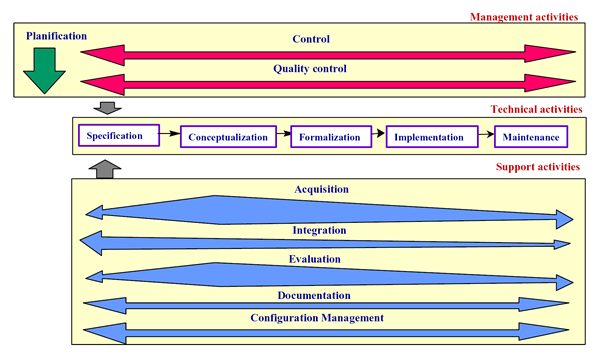
\includegraphics[scale=0.5]{img/methontology_cycle.png}
    \caption{Gambaran tahap-tahap \textit{methontology}}
    \label{fig:Gambar}
\end{figure}

\section{Android}
Android adalah sistem operasi untuk perangkat \textit{mobile} yang dikembangkan oleh Google dengan memanfaatkan \textit{kernel} dari sistem operasi Linux. Sistem operasi ini telah banyak digunakan pada \textit{smartphone}, tablet pc, TV, \textit{wearable device}, dan masih banyak lagi.

Android digunakan sebagai \textit{platform} untuk sisi \textit{front-end} karena kemudahan Android untuk mendapatkan data lokasi pengguna dibandingkan dengan menggunakan PC.

\section{Google Maps API}
Google Maps API \textit{(Application Programming Interface)} adalah sebuah \textit{interface} khusus yang dapat digunakan pengembang perangkat lunak sehingga aplikasi yang dikembangkan dapat menggunakan layanan,fitur dan basis data pada Google Maps.
\par
Google Maps API dipilih karena kemudahan integrasi API pada pengembangan aplikasi Android.  

\section{OpenWeatherMap API}
OpenWeatherMap adalah sebuah API yang menyediakan layanan untuk mendapatkan data cuaca terkini. OpenWeatherMap API memiliki dukungan untuk berbagai macam \textit{platform} seperti Android dan iOS.
\par
Pada tugas akhir ini, OpenWeatherMap akan digunakan untuk mendapatkan data cuaca terkini di lokasi pengguna.

\section{Jython}
Jython merupakan bahasa pemrograman Python yang terintegrasi dengan Java. Berbeda dengan Python biasa yang berjalan dengan \textit{C compiler}, Jython berjalan dengan menggunakan
Java Virtual Machine (JVM). 

\section{Protokol HTTP}
\textit{Hypertext Transfer Protocol} (HTTP) adalah protokol aplikasi yang menjadi dasar komunikasi data pada \textit{World Wide Web}. \textit{Hypertext} adalah teks dengan struktur tertentu yang dikirim diantara \textit{node}. HTTP menjadi protokol agar bisa mengirim \textit{Hypertext}.
\par
HTTP berfungsi untuk memfasilitasi permintaan dan respon data pada model \textit{client-server}. Pada contoh dunia nyata, \textit{web browser} berperan sebagai \textit{client} dengan mengirimkan pesan permintaan HTTP ke \textit{server} yang berperan untuk \textit{hosting}. \textit{Server} akan menyediakan sumber daya yang disebutkan berdasar permintaan HTTP yang diterima dan mengirim respon HTTP kepada \textit{client}.
\par
HTTP memiliki beberapa metode permintaan seperti \textit{GET}, \textit{POST}, \textit{DELETE}, \textit{CONNECT} dan \textit{TRACE}. Metode permintaan yang paling sering digunakan adalah \textit{GET} dan \textit{POST}. Pesan yang dikirim dalam permintaan berisi baris permintaan, \textit{header} dan badan pesan (opsional). Sedangkan respon yang dikirim dengan HTTP berupa kode status permintaan, \textit{header}, dan badan pesan.
\par
Tugas akhir ini menggunakan HTTP sebagai perantara pertukaran pesan antara ponsel pengguna dengan proses yang berjalan pada \textit{server}. HTTP dipilih karena HTTP dapat mengirim pesan dalam berbagai tipe konten seperti teks biasa, html, atau Javascript Object Notation (JSON).   

\section{Javascript Object Notation}
\textit{Javascript Object Notation} atau yang biasa disebut JSON adalah sebuah format pertukaran data. JSON memiliki kelebihan dapat dipahami manusia dengan mudah dan kemudahan \textit{parsing} oleh mesin. 
\newline
Tugas akhir ini menggunakan JSON sebagai format pertukaran data antara \textit{client} dan \textit{web server}.

\section{SPARQL}
SPARQL adalah bahasa \textit{query} untuk basis data \textit{semantic}. SPARQL memiliki kapabilitas membaca dan memanipulasi data yang tersimpan dalam format \textit{Resource Description Framework}(RDF). Data dalam format RDF direpresentasikan dalam bentuk graf. Meskipun begitu, data RDF dapat dikategorikan sebagai database relasional SQL yang menggunakan tiga kolom yaitu subjek, predikat dan objek.
SPARQL akan digunakan untuk menyimpan data \textit{ontology} yang merepresentasikan pegetahuan sistem mengenai lokasi pariwisata Bandung. 
 